\documentclass[UTF8]{ctexart}
\usepackage{graphicx}

\title{杂谈勾股定理}
\author{张三}
\date{\today}



\bibliographystyle{plain}
\begin{document}



\maketitle


\begin{abstract}
这是一篇关于勾股定理的小短文
\end{abstract}

\tableofcontents

\section{勾股定理在古代}
西方称勾股定理为毕达哥拉斯定理,将勾股定理的发现归功于公元前 6 世纪的
毕达哥拉斯学派。该学派得到了一个法则,可以求出可排成直角三角形三边的
三元数组。毕达哥拉斯学派没有书面著作,该定理的严格表述和证明则见于欧几里德\footnote{欧几里德,约公元前 330--275年。}
《几何原本》的命题 47:“直角三角形斜边上的正方形等于两直角边上的两个正方形
之和。”证明是用面积做的。

我过《周髀算经》载商高(约公元前 12 世纪)答周公问:
\begin{quote}
\zihao{-5}\kaishu 勾广三,股修四,径隅五。
\end{quote}
又载陈子 (约公元前 7--6 世纪)答荣方问:
\begin{quote}
\zihao{-5}\kaishu 弱求邪至日者,以日下为勾,日高为股,勾股各自乘,并而开方除之,得邪至日。
\end{quote}
都较古希腊更早。

\section{勾股定理在近代形式}
\bibliography{math}


\begin{figure}[ht]
\centering
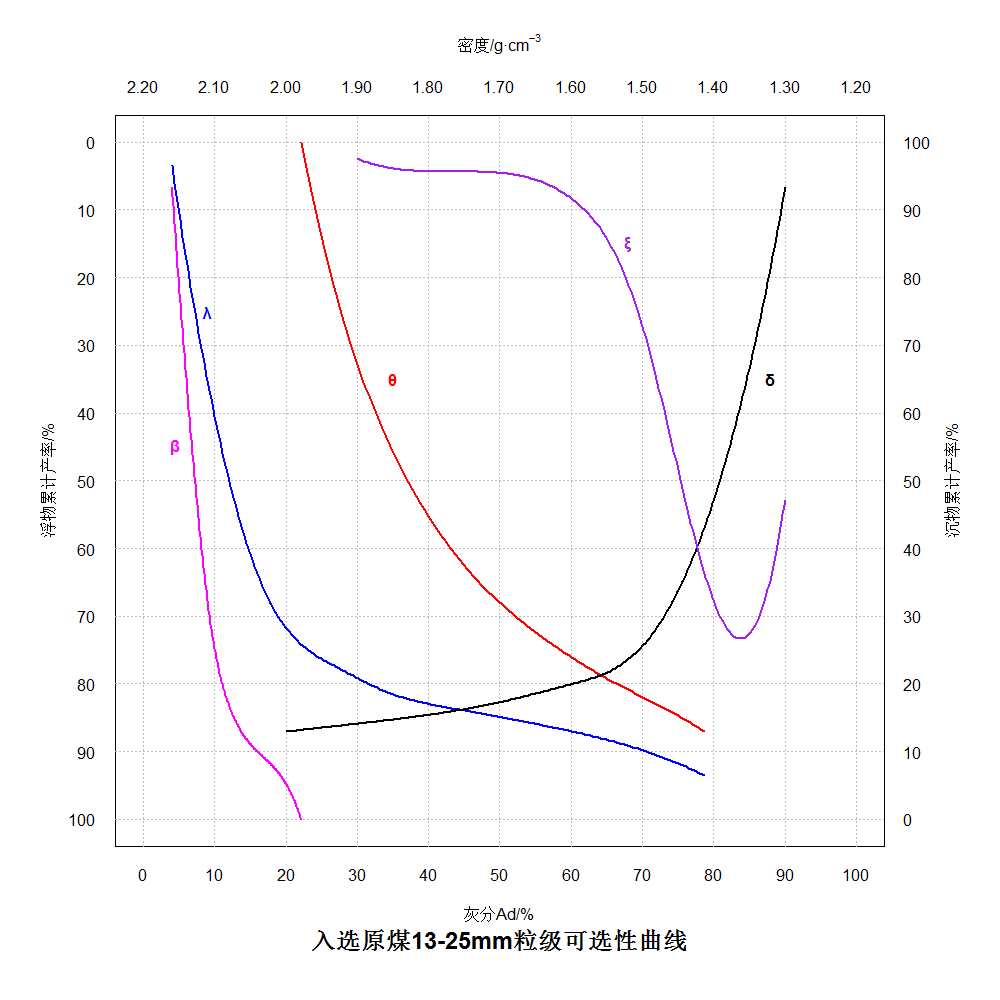
\includegraphics[scale=0.3]{Rplot.png}
\caption{宋赵爽在《周髀算经》注中做的弦图(仿制),该图给出了勾股定理的一个极具对称美的证明。}
\label{fig:Rplot}
\end{figure}

\begin{equation}
a(b+c) = ab + ac
\end{equation}

$\angle ACB = \pi /2 $

\begin{equation}
AB^2 = BC^2 + AC^2
\end{equation}


\end{document}
